%
%		AFIT THESIS MACRO PACKAGE DOCUMENTATION
%                      for version 2.7 of afthesis.cls
%
%
% This file shows the directions of preparing your thesis using the 
% `afthesis' LaTeX document class. This class is an extremely modifed
% `report' document class with new commands added and some old
% commands modified to produce the proper format for the Air Force 
% Institute of Technology thesis or dissertation.
%
% To keep everything simple, this file is designed so that you can use a
% a copy of this file as your LaTeX input file after replacing the
% necessary data by your own data, and inserting your text in the proper
% positions. Inserting text can be done by:
%	-- actually typing the text, or
%	-- using LaTeX \input or \include command
% in the designated position.
% Note that your LaTeX input file name should have the .tex extension, 
% as are the files to be \input'd or \include'd.
%
% The commands \input{foo} inside mythesis.tex will have the effect as 
% if the contents of foo.tex is inserted in the position where the 
% \input command is encountered. To run LaTeX, use the 
% command
%
%	latex mythesis 
%
% To be able to write the inserted text correctly, you are supposed to 
% know basic LaTeX.  All you need to know about LaTeX is written in 
% Leslie Lamport's
% `LaTeX: A Document Preparation System' (Addison-Wesley 1986), which is
% available in local bookstores. 

\documentclass[11pt]{afthesis}
\usepackage{amsmath}
\usepackage{epsfig}
\usepackage{epstopdf}
\usepackage{algorithmic}
\usepackage{algorithm}
\usepackage{amsfonts}

%\documentclass[10pt]{afthesis}  %if you want 10pt instead of 11
%\documentclass[12pt]{afthesis}  %if you want 12pt instead of 11


%\dissertation   % print DISSERTATION instead of THESIS on the title

% Number by chapter ?
%
% You may specify the numbering in your thesis/dissertation to be 
% chapter numbering instead of the default of sequential numbering.  
% If you select this option you will get pages, figures, tables, and 
% equations numbered by chapter (e.g., Table 2.3, Figure 3.4, 
% page numbers 2-40, A-1)
% To not get chapter numbering add a `%' character to the beginning of 
% the next line 

\numberbychapter

% Print section numbers ?
%
% You may select not to have section (and subsection, etc.) numbers 
% printed in the text and in the table of contents. In fact this is 
% the way the AFIT thesis guide shows it, but I like section numbers 
% so I made having section numbers the default.
% To get no section numbers remove the `%' character in the beginning 
% of the next line

%\nosectionnumbers

% Type of empasis ?
%
% You may select to have your emphasized text (like chapter and section
% headings, book titles, foreign phrases, etc.) underlined instead of
% set in an italic font.  By selecting this option, appropriate titles
% are automatically changed, plus anytime you use the command {\em ...}
% you will get underlined text, instead of italic text.  NOTE: this 
% option is not recommended for typeset quality documents. It is here 
% only for those who are old fashioned, type-writer personalities.
% To get underlining instead of italics remove the `%' character in the
% beginning of the next line

%\underlineoption

% Flyleaf frame ?
% 
% You can select to have a 4in by 2in frame put around your flyleaf 
% material.  This makes it look a little nicer if you don't have the 
% cover with the hole in it.
% To get a flyleaf frame remove the `%' character in the beginning of
% the next line.

%\flyleafframe

% Line spacing
%
% The default line spacing is to doublespace except in quotations, 
% quotes, and the bibliography.  This approximates the spacing you 
% get if you "doublespace" on a typewriter.  If you want to change 
% the line spacing use the command \spacing{n} where n is a real 
% number at the start of the document and \endspacing at the end 
% of the document. Use 1 for n to get singlespacing, 1.5 for space 
% and a half, etc.  If you want to change the linespacing to 
% singlespace for a particular section of text, you can use the 
% singlespace environment bracketting your text with 
% \begin{singlespace} and  \end{singlespace} \spacing{2} is the 
% default line spacing for the thesis in 10pt \spacing{1.5} is the 
% default line spacing for the thesis in 11pt and 12pt
%
%  THE ABOVE LINE SPACING INFORMATION IS NOT QUITE ACCURATE
%
% Data of author and thesis: The following data will be used throughout
% your thesis when they are needed. Please replace the dots in the
% commands by your own data. For some commands, the specified default
% value will be assumed when the command is omitted.  For a two author
% thesis, specify the command \twoauthor and then enter the appropriate
% additional fields.  Remember you will need two vitas specified in
% author order.  Authors should be specfied in alphabetical order.

\author{Justin Fletcher}


\rank{First Lieutenant, USAF}

\title{ANISOTROPIC SIMULATED ANNEALING AND ITS APPLICATION TO FEED FORWARD NEURAL NETWORK WEIGHT SELECTION}

%\flytitle{...}
%
% Remove the % and replace the dots in the above command with your
% thesis title as it should be on the flyleaf.  This is only needed
% if your flyleaf title has different line breaks 
% (because it must fit in 4 inches)
% than the way it appears on the title page and on the first page.

\designator{AFIT/GE/ENG/16-..}
%
% Replace the dots in the above command with the thesis or dissertation
% designator. For example, `AFIT/GCS/ENG/87-5'.

%\distribution{...}
%
% Replace the dots in the above command with the distribution
% statement for your thesis.  The default if commented out is 
% `Approved for public release; distribution unlimited'.

\previousdegrees{B.S. CEC}
%\previousdegreestwo{...} %uncomment for twoauthor option
%
% Replace the dots in the above command with the 
% abbreviated form of your previous degree(s), e.g., B.S. or B.A., M.S.
% Leave this command out if you have no previous degrees.

\degree{Master of Science in Computer Science}
%
% The degree sought as determined by your program. 
% For example, `\degree{Master of Science}', or
% `\degree{Master of Science in Electrical Engineering}'.
% The default value is `Doctor of Philosophy' for dissertation.

\graduationdate{June, 2016}
%
% Replace the dots in the above command with the 
% graduation date, in the form as `\graduationdate{May, 1986}'.
% The default value is guessed according to the time of running LaTeX.

\address{452 Orchard Drive\\Oakwood, Ohio 45419}
%\addresstwo{...\\...} %uncomment for twoauthor option
%
% Replace the dots in the above command with your permanent address.
% Use \\ to separate address lines.  This is used in the Vita.
% e.g., `\address{4533 Avenue A\\ Austin, Texas 78751}'.

\school{Electrical and Computer Engineering}
%
% Replace the dots in the above command with the name of your school.  
% For example, `\school{School of Engineering}'

%**********for dissertations only, remove the % signs and add the data
%\dean{...}
% Needed for disserations only.
% The name of your dean, e.g., `\dean{Robert A. Calico, Jr}

\committee{Dr. Michael J. Mendenhall\\Thesis Advisor,
	Dr. Gilbert L. Peterson\\Committee Member,
	Capt. Charlton D. Lewis, Ph.D.\\Committee Member}
% 
% The default value is 5 for dissertation. 

\begin{document}
	
	% The following commands will automatically generate headings, adjust
	% vertical spacings, break pages, etc.
	% You should probably leave all of these prefatory pages commented out
	% or in a \include file until your thesis is ready for final draft
	
	\flyleaf      			% Generates the flyleaf.
	
	\disclaimerpage                 % Produces the disclaimer page
	
	\titlepage			% Produces the title page.
	
	\approvalpage                   % Produces the approvalpage
	
	\begin{preface}
		%
		%Insert the text of your preface here. Your name will appear
		%automatically. If this is an acknowledgments section instead of 
		%preface, use \begin{acknowledgments} and \end{acknowledgments}
		% instead.
		%
	\end{preface}
	
	\tableofcontents	% Table of Contents will be automatically
	% generated and placed here.
	
	\listoffigures  	% List of Figures, List of Tables, and List of
	\listoftables		% Symbols will be placed here, if applicable.
	\listofsymbols      % Do not use these if you have no such lists.
	% To put symbols in the list use command \symbol[#1]{#2}
	% where #2 is the symbol and #1 is the definition to be put in the
	% list of symbols. The symbol is also automatically put in
	% your text.  Leave out [#1] if you don't want a definition.
	
	\listofabbreviations
	
	\abbreviation[Artificial Neural Network]{ANN}
	% similar to the list of symbols.  Use command \abbreviation[#1]{#2}
	% where #2 is the abbreviation and #1 is the definition to be put in the
	% list of abbreviations. The abbreviation is also automatically put in
	% your text.  Leave out [#1] if you don't want a definition.
	
	\begin{abstract}
		% Lower-end page count: 131
		% Upper-end page count: 170
		% DO: Write abstract.	
		Stub.
	\end{abstract}
	
	
	\chapter{Introduction}
	
	% DO: Write introduction.	
	% The first chapter. \chapter command is of the form \chapter[..]{..} or \chapter{..} where {chapter heading} and [entry in table of contents].
	
	% Do this after the thesis is written. I created an algorithm which simulates quantum tunneling through an error manifold. I applied this algorithm to the problem of selecting weight values for a neural network. It works well for small data sets, but is slower when dimensionality of the data set on which the network is trained is very large. 
	
	
	Stub.
	
	% In chapter three the traversal a error manifold in the problem configuration space is discussed at length. Several traversal methodologies are proposed and evaluated. 
	
	
	% Important: If your chapter heading consists of more than one lines, it will be automatically broken into separate lines. However, if you don't like the way LaTeX breaks the chapter heading into lines, use `\newheadline' command to break lines. NEVER USE \\ IN SECTIONAL (E.G., CHAPTER, SECTION, SUBSECTION) HEADINGS!!!!!!!!
	
	\chapter{Background} % This is Chapter 2.
	
	This chapter serves as a comprehensive review of the physical and computational concepts material to the topic of this thesis. A broad overview of artificial neural networks and the application and history thereof is presented. Next, various formulations of simulated annealing are described, along with a summary of some related works and a description of the physical inspiration for the algorithm. The chapter concludes with a very brief overview of the quantum mechanics, with emphasis placed on those concepts which will be employed throughout the document. Finally, the notation and terminology conventions adopted in this thesis are established.
	
	\section{Artificial Neural Networks}
	
	% Is there a better term than sequential computing machinery? 
	
	% Each word in this name encodes a significant concept related to the origins and structure of the models: neural is a reference to neurons, which are the fundamental information processing elements of the biological systems which inspired the model; network refers to network theory, a subfield of graph theory, which governs representation of relationships between neurons; and artificial, meaning an object of human origin, in contrast with biological neural networks which arise naturally.
	
	It has long been recognized that the capacity of biological information processing systems to flexibly and quickly process large quantities of data greatly exceeds that of sequential computing machinery. This information processing capability arises from the complex, nonlinear, parallel nature of biological information processors. The family of models designed to replicate this powerful information processing architecture are collectively called artificial neural networks (ANNs). In the most general sense, ANNs are parallel distributed information processors \cite{haykin1999} comprising many simple processing elements. Networks store information about experienced stimuli in the form of connection strengths and network topology and can make that information available. In such a network, interneuron connection strengths are used to encode information, and are modified via a learning strategy. ANNs are characterized by three features: a network topology or architecture, an activation function, and a learning strategy; each is discussed in the following sections. Additionally, an abbreviated history of ANNs is provided and the biological inspiration for the computational model is described.
	
	\subsection{Biological Inspiration}
	
	This is all one big stub.
	
	Fig[an image of a neuron, mapped to a schematic of a neuron, mapped to a processing element]
	
	Integration of magnitude-encoded, rather than frequency-encoded, signals. 
	Threshold functions relationship to the biological shape, size... Papers needed.
	
	Biological neural networks are many orders of magnitude slower than those based in ... It in not the size of the network or the number of interconnections alone which confer upon the human brain its remarkable efficiency (Faggin, 1991). Though size and connectivity are necessary, it is the structure, or topology of the network of interconnections that en
	
	% What is the physical mechanism for synaptic depression? Flooding of synaptic cleft with inhibitory neurotransmiters?
	
	Activation time-line: The concentration of neurotransmitters in the extra-synaptic fluid increases, raising the instantaneous membrane potentiality, possibly breaching the threshold potential causing a fire-and-reset, where the there is some physical limit on the rate at which the reset step can occur, thus causing the diminishing response seen in Figure 2 of Neurocomputing, whence the fire causes either excitatory or depressive neurotransmitters to be released at the synaptic clefts formed at the end of the axon, thus propagating the activation through the net.
	
	What is changed in synaptic modification is the efficiency with which a particular post-synaptic site is able to convert neurotransmitters in the surrounding intercellular environment, which is to say in the synaptic cleft, into a change in charge inside the cell.
	
	Activation function: A neurons activation function is just a phenomenon emerges from from the combination of its potential threshold and rest rate, both of which are physiological properties which can change after cell formation. (Instructing Perisomatic Inhibition by Direct Lineage Reprogramming of Neocortical Projection Neurons, 2015)
	
	\subsection{Historical Overview}
	
	
	% Pre-1970
	The study of ANNs began with a 1943 paper \cite{mcculloch1988} by McCulloch and Pitts. In this paper, McCulloch and Pitts united, for the first time, neurophysiology and formal logic in a model of neural activity. This landmark paper marked the beginning of not only the computational theory of neural networks but also the computational theory of mind, and eventually led to the notion of finite atomata \cite{piccinini2006}. In  \cite{mcculloch1988} McCulloch and Pitts introduced a very simple model of a neuron, which acted as a threshold-based propositional logic unit. Significantly, McCulloch and Pitts showed that a network of their neuron models, interconnected, could represent a proposition of arbitrarily-high complexity. Said differently, a network of the neuron models described in  \cite{mcculloch1988} can represent any logical proposition. These models are often called McCulloch-Pitts neurons and permit only discrete input values which are summed and compared to a threshold value during a fixed time quantum, and do not posses any learning mechanism.  McCulloch-Pitts neurons are able to incorporate inhibitory action, but the action is absolute and inhibits the activation of the neuron without regard to any other considerations. The McCulloch-Pitts neuron model is of theoretical significance, but cannot be applied to practical problems.
	
	%[Graphic Stub: Simple McChulloch-Pitts neuron.]
	
	% DO: This paragraph needs rework around the work effeciency.
	Though McCulloch and Pitts made mention of learning in their 1943 paper, thirteen years would pass before the learning concept was formalized into a mathematical and computational model. In 1956 Rochester, Holland et. al. \cite{rochester1956} presented the first attempt at using a physiologically-inspired learning rule to update the synaptic weights of a neural network. This model was based on the correlation learning rule postulated in 1949 by Hebb\footnote{It should be mentioned that, while Hebb was the first to postulate the correlation learning rule as it relates to neurons and synaptic connection strength, the abstract rule was foreshadowed as early as 1890 by William James \cite{james1890principles} in Chapter XVI of \textit{Psychology (Briefer Course)}.}. In his book \textit{The Organization of Behavior}, Hebb suggested that synaptic plasticity, that is the capacity of synaptic strengths to change, is driven by metabolic and structural changes in the both neurons near the synaptic cleft \cite{hebb1967} such that if two cells often fired simultaneously the efficiency with which they cause one another to fire will increase. This efficiency is now called a synaptic weight. Rochester et. al. showed that the addition of variable synaptic weights alone was not sufficient to produce a network capable of learning; the weights must also be capable of assuming inhibitory values.
	
	% DO: is this paragraph too detailed, or not detailed enough? 
	% DO: Quick graphic of the perceptron.
	
	[Graphic Stub: simple perceptron terminology, figure.]
	
	The next major contribution to the field would come in 1958 with Rosenblatt's introduction of the simple perceptron \cite{rosenblatt1958perceptron}. The perceptron was the first \cite{anderson1988neurocomputing} well formed, computationally oriented neural network. Crucially, and unlike most preceding neural models, the model Rosenblatt presented in his  1958 paper was associative. That is, the model learned to associate stimuli with a response. This learning is accomplished by modifying the synaptic weights of the model such that the difference between an input pattern and the desired output pattern is minimized. The responsibility for the error, or difference between the correct and computed output patterns, is divided among the weights in proportion to their magnitude. Thus, large synaptic weights will be reduced more than small synaptic weights for a large, positive error. This weight update strategy is represented mathematically as: \begin{equation} 
	w_i(t+1) = w_i(t) + \alpha(d_j - y_j)x_{j,i}
	\end{equation} where \begin{math} w_i(t) \end{math} the synaptic weight for feature \begin{math} i \end{math} at discrete time \begin{math} t \end{math}, \begin{math} \alpha \end{math} is the tunable learning rate parameter, \begin{math} d_j \end{math} is the desired output, \begin{math} y_j \end{math} is the computed output, and \begin{math} x_{j,i} \end{math} is the input pattern. This method constitutes a from of reinforcement learning.
	
	
	% DO: is corollary appropeiate here? 
	Rosenblatt's perceptron was found to be successful at predicting the correct response class for stimuli only if the responses were correlated. It was not until Block's 1962 publication that the reason for this observed performance was elucidated. In this paper, Block presented two key findings: first, that simple perceptrons require linearly separable classes to achieve perfect classification and second, the perceptron convergence theorem \cite{block1962perceptron}. Linear separability is the ability of the response classifications to be separated by a hyperplane in the \begin{math}n\end{math}-dimensional space of the input stimuli to which they correspond. The requirement of linear separability arises directly from the way in which the output of a perceptron response unit is calculated. The output of a perceptron response unit is given by:
	\begin{equation} 
	y_j = \begin{cases}
	-1 &\sum_{i=1}^{n} w_{i,j}x_{i} \leq \Theta\\
	+1 &\sum_{i=1}^{n} w_{i,j}x_{i} > \Theta
	\end{cases}
	\end{equation} where \begin{math} y_j \end{math} is the response value of response unit \begin{math} j \end{math}, \begin{math} w_{i,j} \end{math} is the synaptic weight of the connection between activation unit \begin{math} i \end{math} and response unit \begin{math} j \end{math}, \begin{math} x_{i} \end{math} is the activation value of activation unit \begin{math} i \end{math}, and \begin{math} \Theta \end{math} is the threshold value of the perceptron. Block's crucial observation was that the form of the summation in the response determining equation is isomorphic to a hyperplane in an \begin{math}n\end{math}-dimensional space. Thus, in order for the perceptron to achieve perfect classification, a hyperplane must be able to separate them in the \begin{math}n\end{math}-dimensional input space. The corollary of this observation it the perceptron convergence theorem. The theorem proves that for some learning rules, if a perfect classification is possible it will be found by the perceptron. Specifically, the class of learning rules which were found effective were those which did not change synaptic weights when a correct classification occurs. While the condition does ensure convergence, it often causes very slow convergence, as the synaptic weights change much more slowly when only a small number of samples remain misclassified. Considerably faster guaranteed convergence can be achieved using a error gradient descent learning rule \cite{widrow1960asc}, as described by Widrow and Hoff. 
	
	% DO: This paragraph is a little light on details, but it's either all or none, so if more is needed, I can add it.
	In 1969 Minksy and Papert published \textit{Perceptrons}, a book on mathematics and theory of computation. In this book Minsky and Papert mathematically and geometrically analyzed the limitations inherent in the perceptron model of computation. The authors reasoned that the each response unit of Rosenblatt's perceptrons was actually computing logical predicates about the inputs it received, based on the observation that response units can either be active or inactive. This analytical framework allowed the authors to construct unprecedented geometric and logical arguments about the computational capabilities of a perceptron. They found that there were several classes of problems which were unsolvable by linear perceptrons \cite{minsky1969perceptrons}. In the final chapter of the \textit{Perceptrons} Minsky and Papert extended their judgments regarding the ineffectiveness of single-layered perceptrons to all variants of perceptrons, including the multi-layered variety. This conjecture would turn out to be one of the most significant of the entire book, as it likely resulted in a reduction of funding for neural network research \cite{anderson1988neurocomputing} which lasted for several years. Unfortunately, this judgment was incorrect.
	
	% 1970-1980
	While it is true that the pace of development in the field of neural networks slowed considerably after the publication of \textit{Perceptrons}, there was still progress made during the 1970s. In 1972, both Anderson \cite{anderson1972interactive} and Kohonen \cite{kohonen1972correlation} published models of what would come to be known as linear associative neural networks, which are a generalization of Rosenblatt's perceptron. As with the perceptron, neurons in a linear associative neural network compute their output by summing the product of each input signal the synaptic weight associated with that input. Unlike the perceptron, the output of these networks is proportional to this sum, rather than a binary value computed by applying a threshold function to the sum. Though still unable to achieve perfect classification on many classes of problems, these networks were able to successfully associate input patterns with output patterns. 
	
	% DO: Much more data can be added to this paragraph.
	The decade also saw the advent of self-organized maps, which are a type of competitive learning neural network. Self-organization in neural networks was first demonstrated by van der Malsburg in a paper \cite{vonderMalsburg1973selforganization} published in 1973. This paper analyzed the response of simulated cortical cells to a simulated visual stimulus. The paper is interesting both for the complexity of the neural model developed, and because it contained the first direct comparison between computer simulation and physiological data \cite{anderson1988neurocomputing}. 
	
	% DO: I'm not exactly sure  how to handle this data. It seems to contradict the claim of the essenital nonlinear nature of neural nets.
	Throughout the decade progress was also made in the understanding of the physiology of biological neural networks. Of particular interest are those papers describing the lateral retinal system of \textit{Limulus polyphemus}, the horseshoe crab. Chosen for the easy with which experiments may be conducted on its compound lateral eye, \textit{Limulus} features prominently in the neurophysiological research. Several works were published on the \textit{Limulus}, perhaps the most significant of which came near the end of the decade with the 1978 publication of a paper describing the dynamics of the retina of a \textit{Limulus} when exposed to moving stimuli. In this paper,  the \textit{Limulus} eye was analyzed as a linear system, and the results of this analysis were compared to the actual response of the system to input pattern. The agreement between the linear\footnote{Linear, in this context of this system, means that the output of the system when presented with the sum of a set of inputs is equivalent to the sum of the outputs of the system when presented with each input individually.} model and the biological output signals was found to be in excellent agreement \cite{brodie78limulus}. This finding was interesting for the purposes of perceptron simulation, but was ultimately found not not to hold for larger collections of neurons. %(NEED SOURCE...)
	% post-1980
	
	%"Likelyhood of escpae graph"
	%"Relative likelyhood of escape graph"
	%"Projection from color on the PES to an independent graph"
	%"learn rate on PES with simulated annealing is just like downsampling the sapce and searching the downsampled space. Add stochat"
	% Simultaneously anneal topology, weights, and activation functions. How do you define distance in this configuration space which includes both discretes and reals?
	
	Several events conspired to create a reinvigoration of neural network research in the early 1980s. Theoretical advances in the physiology of biological neural networks. processor manufacturing technology had advanced sufficiently to allow for much larger-scale simulations.  simulation capability...
	
	In 1982, John Hopfield published \textit{Neural networks and physical systems with emergent collective computational abilities}. This momentous work is regarded by many to be the beginning of the renaissance of neural network research \cite{anderson1988neurocomputing}, and contains many novel insights. Hopfield begins the paper differently than past researchers. Rather than proposing a learning rule or network topology and then evaluating the results of this proposition, Hopfield begins by considering an alternative purpose for a neural network. Hopfield suggests that the network be thought of as a means to develop locally stable points, or attractors, in a state space. The state space comprises the set of states which are the activation value of each neuron. Thus, learning should be the process of modifying the synaptic weights such that they cause the system to flow into local attractors which represent the desired output. In such a model, a noisy or incomplete input would result in an activation pattern which resides on a gradient in the state space. The neural network would then change the activation pattern in such a way as to move the system down the gradient into the attractor state. Hopfield suggests that this process is a general physical description of the concept of content-addressable memory.
	
	% DO: Produce, in Julia, a 2d 2-minima plot.
	[Graphic Stub: notional activation state space with letters and noisy letters as points.]
	
	Hopfield then proposes a network architecture to achieve this behavior \cite{hopfield1982neuralnetworks}. The chosen model is one which has binary neural output values and recurrent connections. Neural networks of this types are now called Hopfield networks. Like Rosenblatt's original perceptron model, the neurons used in Hopfield's work had a non-linear, threshold activation function. The network topology was recurrent, with the restriction that no neuron could provide input to itself. Hopfield adopted a variation of Hebb's learning rule to update the synaptic weights.
	
	In Hopfield's network model, the connection strength between two neurons \begin{math}i\end{math} and  \begin{math}j\end{math} is denoted as \begin{math}T_{ij}\end{math}, and the activation status of a neuron \begin{math}i\end{math} is denoted as  \begin{math}V_i\end{math}. \begin{math}T\end{math} is therefore the connection matrix of the neural network, with each element representing an individual connection strength and zeros along the diagonal. It is from this organization of the connection strengths that one of the most important insights of this work originates. Hopfield recognized that, in the special case of the model in which \begin{math}T_{ij}=T_{ji}\end{math}, a quantity \begin{math}E\end{math} could be defined such that \begin{equation} 
	E= -\frac{1}{2} \mathop{\sum\sum}\limits_{i \neq j} T_{ij} V_i V_j .
	\end{equation} The change in this quantity as a result of a change in one of the activation values, \begin{math}V_i\end{math} in the following equation, is then represented as \begin{equation} 
	\Delta E= -\Delta V_i  \sum\limits_{j \neq i} T_{ij} V_j .
	\end{equation} From this equation, it is clear that any change in \begin{math}V_i\end{math} will reduce the value  of \begin{math}E\end{math}. This decrease in \begin{math}E\end{math} must necessarily continue until some local minimum of the value of \begin{math}E\end{math} is reached\footnote{An identical conclusion would be reached if \begin{math}V_j\end{math} was changed instead of  \begin{math}V_i\end{math}. It is merely a matter of convention.}. Here, Hopfield observed that this case is isomorphic with an Ising model," referencing the statistical mechanical model of magnetic spins. In this isomorphism, the quantity \begin{math}E\end{math} maps to the energy of a physical system described by an Ising model. It is difficult to overstate the importance of this observation. It both provided a novel mechanism by which physical theory could be applied to neural networks, and legitimized the study of neural networks as a physical system, encouraging many physicist to join in the development of the theory.
	
	Hopfield constructed a model of the system described in the paper, and presented it with random input patterns\footnote{Hopfield calls these input patterns entities or \textit{Gestalts}.}. He found that the network can indeed recall a small number of patterns, on the order of approximately 15 percent of the network dimensionality, before the recall error becomes significant.
	
	In 1985, Ackley et. al. extended the neural network model proposed by Hopfield\footnote{Though a Hopfield network was used for the work done by Ackley, Hinton, and Sejnowski it is not necessary to use network with recurrent connections.}. Hopfield networks are deterministic with respect to energy; by definition any change in a Hopfield network always reduces the energy of the system or leaves it the same. This is a useful property if it is acceptable to find one of many local minima, or attractors. However, if a single, global minima in the state space is sought this model is likely to converge prematurely to a local attractor state. In order to surmount this limitation Ackley et. al. modified the Hopfield neural model to activate stochastically. The probability of state transition, \begin{math}p\end{math}, is given by \begin{equation} \label{eq:boltzmannProb}
	p= \frac{1}{1 + e^{- \Delta E  / T} }
	\end{equation} where \begin{math} \Delta E \end{math} is the change in energy of the system resulting from a transition to a new state and \begin{math}T\end{math} is the artificial temperature of the system. Thus the relative probability, \begin{math}P_{\alpha}/P_{\beta}\end{math} of moving to either of two arbitrary global states, \begin{math}\alpha\end{math} and \begin{math}\beta\end{math}, is defined as \begin{equation} \label{eq:boltzmannDist}
	\frac{P_{\alpha}}{P_{\beta}} =  e^{- (E_{\alpha} - E_{\beta} ) / T} 
	\end{equation} which is a form isomorphic to the Boltzmann distribution. Thus, a neural network with transition probabilities described by equation \ref{eq:boltzmannProb} is called a Boltzmann machine. The effect of probabilistic state transitions of this form is that state transitions from low energy states to higher energy states are possible, thereby allowing the system to escape local minima. 
	
	Inspection of equations \ref{eq:boltzmannProb} and \ref{eq:boltzmannDist} reveals that the probability of transition is determined by both \begin{math}\Delta E\end{math} and \begin{math}T\end{math}. A large value of \begin{math}\Delta E\end{math}, which corresponds to a large increase in total energy, will decrease the probability of transition. Conversely, a large value of \begin{math}T\end{math} will increase the probability of transition for any arbitrary value of \begin{math}\Delta E\end{math}. The systems artificial temperature therefore acts as a tuning mechanism for the exploration of the state space. A high temperature value will result greater exploration of the space state, but will result in less gradient descent and therefore may cause the system to depart the attractor basin of the global minimum. A low artificial temperature parameter may cause premature convergence. Ackley et. al. solved this tuning problem by recognizing a deep connection to another concept born of statistical mechanics: simulated annealing. Simulated annealing decreases the artificial temperature of a system slowly over the course of a simulation, and as a result increases the likelihood that the final state of the system will be the ground state, which is to say the global minimum. This algorithm is discussed in detail in section \ref{eq:simulatedAnnealing}.
	
	% DO: Could use a better source here
	With a procedure for finding the global minimum of a space state in place, the authors proceeded to construct state spaces for which the global minimum was of interest. One way to construct such a state space is to include hidden units in the neural network. Hidden units are neural units which are neither input nor output units. These hidden units allow the network to solve interesting problems that are out of reach of simple associative neural networks\cite{anderson1988neurocomputing}. However, like all neurons in any neural network, the connection weights of these neurons must be modified in order for the network to learn. It is not immediately clear how hidden unit synaptic weights can be modified to account for the performance of the network. This deficiency is often called the credit assignment problem\cite{barto1983neuronlike}. The application of simulated annealing in Boltzmann machines avoids the problem of assigning credit to hidden units, thereby enabling their inclusion in the model. This is historically significant because it was the first successfully-implemented multi-layered neural network \cite{haykin1999}.

	The next major development in neural networks came in 1986 with the introduction of the back-propagation algorithm. Though the formalisms required involved in this algorithm had been developed earlier \cite{bryson1969optimalcontrol} \cite{werbos1974beyondregression}, and the method was simultaneously discovered independently by two other groups \cite{parker1985logic} \cite{lecun1985}, it was Rumelhart et. al. that applied the algorithm to machine learning \cite{rumelhart1986internal}. Back-propagation can be thought of as a generalization of the gradient descent\footnote{The gradient descended in this context is the gradient of the error surface in the space of states of synaptic weights, not the gradient of the activation state surface, as with a Hopfield network.} algorithm presented by Widrow and Hoff \cite{widrow1960asc}, which includes the errors associated with connection strength of hidden units, or internal representation units. A detailed discussion and derivation of the back-propagation algorithm is included in Section \ref{sec:backpropTraining}. Though back-propagation in multilayered perceptrons cannot be guaranteed to find an exactly correct solution, the algorithm is demonstrably capable of solving difficult and interesting problems, thus disproving the speculation of Minsky and Papert in \cite{minsky1969perceptrons}.
	
	% ...The utility of back propigation lies in its relative computational effeciency; though both back-propigation and simulated annealing can be used to select the synaptic weights for a neural network, back-propigation generally converges to a solution several orders of magnitude faster ()
	
	With the advent of Boltzmann machines and back-propagation, it became possible to analyze the properties and capabilities of multilayered neural networks. In 1989 Cybenko showed that a multilayer feedforward neural network with nonlinear activation function is in principle capable of approximating any continuous function  \cite{cybenko1989approxsuperposition}. This finding is striking because it implies that, given the correct learning rule and a sufficiently large network, a multilayer neural network can learn a pattern of arbitrary complexity. 
	
	
	%This, in turn, implies that neural networks can serve as universal function approximaters. (Cybenko1989)
	
	%(Kurt Hornik (1991) "Approximation Capabilities of Multilayer Feedforward Networks", Neural Networks, 4(2), 251–257)
	
	
	
	
	
	\subsection{Network Topology}
	
	Stub.
	
	%The topology of a neural network describes the way in which the individual processing units are interconnected. There are only a few broad classes of topology, each of which has different properties. 
%	Feed forward
%	recursive
%	recapitulated backprop here...
	\subsection{Activation Functions}
	
	Stub.
	% DO: Proof of the necessity of non-linearity.
	% DO: Any work on variable activation functions?
	
	\subsection{Learning Strategies}
	
	Stub.
	
	%General discussion.
	
	%Reference (Mendel and McClaren, 1970) and (Haykin, pg 50)
	
	
	\subsubsection{Back Propagation Training} \label{sec:backpropTraining}
	Stub.
	
	% DO: Consider pandimonium by slefedger
	
	% DO: Discuss (Rumelhart, Hinton, Williams, 1986)
	
	% DO: Derive back prop. (Haykin, pg 161)
	
	% DO: Discuss the implication of local minima.
	
	% DO: Fig[Error surface with backprop]
	
	
	\subsubsection{Simulated Annealing} 
	Stub.
	
	
	
	\section{Related Works in Simulated Annealing} \label{eq:simulatedAnnealing}
	
	% DO: Read (Haykin pg 556)
	
	% DO: Read (Haykin pg 560)
	
	Simulated annealing (SA) is a stochastic optimization algorithm which can be used to find the global minimum of a cost function mapped from the configurations of a combinatorial optimization problem. The concept of simulated annealing was introduced in by Kirkpatrick et al. in \cite{kirkpatrick1983} as an application of the methods of statistical mechanics to the problem of discrete combinatorial optimization. Specifically, simulated annealing is an extension of the Metropolis-Hastings \cite{metropolis1953} algorithm which can be used to estimate the ground energy state of a many-body systems at thermal equilibrium. Kirkpatrick et al. applied the Metropolis-Hastings algorithm sequentially, with decreasing temperature values in order to approximate a solid slowly cooling to low temperatures. Later work by Goffe \cite{goffe1994globaloptimization}, Corana et al. \cite{corana1987minimizingmultimodal}, and Lecchini-Visintini et. al. \cite{lecchinivisintini2007sacontinuousgaruntees} extended SA to the continuous domain.
	
	In the most general terms, SA is a local search algorithm through the problems solution space, \begin{math} \boldsymbol{\mathcal{S}} \end{math}, which is the set of all possible solutions, \begin{math}\boldsymbol{s}  \end{math}, of the problem. The search is conducted by generating new solutions to the problem by applying a neighborhood function, \begin{math}\boldsymbol{\mathcal{N}} \end{math} to the current solution; the neighborhood function specifies the way in which a solution is transformed to yield a new solution, or neighbor solution, and is generally problem dependent. To apply SA to an optimization problem it must be possible to characterize each possible solution of the problem using a cost function, \begin{math}\mathcal{C} \end{math}, where \begin{math}\mathcal{C} \end{math} is the mapping
	
	\begin{equation*} \label{eq:cost_mapping}
	\mathcal{C} : \boldsymbol{\mathcal{S}} \rightarrow \mathbb{R}.
	\end{equation*}
	
	\noindent Because \begin{math} \mathcal{C} \end{math} is a function on \begin{math} \boldsymbol{\mathcal{S}} \end{math}, it is said that the cost function forms a cost surface in the solution space. During each iteration of the algorithm, a new solution, \begin{math}\boldsymbol{s}'  \end{math}, is generated using \begin{math}\boldsymbol{\mathcal{N}(\boldsymbol{s})} \end{math}, and the cost of that solution, \begin{math}\mathcal{C}(\boldsymbol{s}' ) \end{math}, is determined. The change in cost associated with moving from the current solution to the neighbor solution is given by 
	\begin{equation*} \label{eq:delta_cost}
	\Delta C =  \mathcal{C}(\boldsymbol{s}')-\mathcal{C}(\boldsymbol{s}).
	\end{equation*}
	
	\begin{math}\Delta C \end{math} is then used in conjunction with an artificial temperature parameter to determine if the newly-generated neighbor solution is to become the current solution. The artificial temperature parameter is specified by the temperature schedule, \begin{math}T(t)\end{math}, where \begin{math}t\end{math} is the number of simulation iterations completed. The temperature controls the probability of the system moving to a higher cost solution, thereby enabling the algorithm to escape local minima on the cost surface. In the parlance of SA \cite{kirkpatrick1983} a system at its maximum temperature is said to be \textit{melted}. In the melted state, most neighbor solutions are accepted by the algorithm. Analogously, a system that has a temperature of zero, which indicates that the algorithm cannot move to any higher-error state, is said to be \textit{frozen}. Note that a frozen system may still be perturbed into a lower-energy state. The notions of freezing and melting enter the SA algorithm in the form of the acceptance criterion, which determines if a newly-generated solution is to become the current solution. The most commonly used acceptance criterion is the Metropolis criterion \cite{metropolis1953}, given by:
	
	\begin{equation} 
	y_j = \begin{cases}
	1 &\Delta C   \leq 0 \\
	e^{-\frac{\Delta C}{T(t)}} & \Delta C > 0 
	\end{cases}
	\end{equation}

	
	The probability of moving to a solution which is higher in cost than the current solution is derived from the statistical mechanical probability of traversing a potential energy barrier by thermal fluctuations. When considering only the influence of classical thermal fluctuations in particle energy levels, the probability of a particle traversing a barrier of height \begin{math} \Delta V \end{math} at a temperature \begin{math} T \end{math} is on the order of: \begin{equation} 
	\mathcal{P}_t = e^{-\frac{\Delta V}{T}} 
	\label{eq:thermal_traversal_prob}
	\end{equation}
	
	 The SA algorithm is presented in Algorithm~\ref{alg:simulated_annealing}. 



	% The physical inspiration for simulated annealing. See (Haykin pg 546)
	
	\begin{algorithm}
		\caption{Simulated Annealing}
		\label{alg:simulated_annealing}
		\begin{algorithmic}
			\STATE $\boldsymbol{s} \leftarrow \boldsymbol{s}_0$
			\STATE $t \leftarrow 0$
			\WHILE{$T(t) > \epsilon$}
			\STATE $\boldsymbol{s}' \leftarrow \boldsymbol{\mathcal{N}}(\boldsymbol{s}) $
			\STATE $\Delta C \leftarrow (\mathcal{C}(\boldsymbol{s}')-\mathcal{C}(\boldsymbol{s}))$
			\IF{$\Delta C \leq 0 $}
			\STATE $\boldsymbol{s} \leftarrow \boldsymbol{s}'$
			\ELSE [$ \exp(\Delta C/T(t) ) > U\left( 0,1\right)  $]
			\STATE $\boldsymbol{s} \leftarrow \boldsymbol{s}'$
			\ENDIF
			\STATE $t \leftarrow t+1$
			\ENDWHILE
			\STATE $\boldsymbol{s}_{opt} \leftarrow \boldsymbol{s}$
			\RETURN $(\boldsymbol{s}_{opt})$
		\end{algorithmic}
	\end{algorithm}
		
	We need here a discussion regarding the asymptotic convergence.
	
	In \cite{szu1987fastsimulatedannealing} Szu and Hartley introduced the method of fast simulated annealing (FSA), which incorporates occasional, long jumps through the configuration space, These jumps are accomplished by using a heavy-tailed distribution, such as the Cauchy distribution, for the visiting distribution used in the neighborhood function. This provision increases the likelihood of escaping local minima, and reduces the total computational effort required to reach a global minimum. This modification yields a significant decrease in the amount of computation effort required to guarantee that a global minimum is found. Specifically, the FSA decreased the required temperature decay from $1/\ln(t)$ to $1/t$, where $t$ is the simulation time. Later work by Tsallis and Stariolo \cite{tsallis1996generalizedsimulatedannealing}, generalized both CSA and FSA into a single framework: generalized simulated annealing (GSA), which was faster still.
	
	% Be sure to include some discussion of thermal fluctuations and their importance. Find a nice source...
	\subsection{Reheating}
	Stub.
	
	
	\section{Related Works in Quantum Mechanics}
	
	
	Quantum mechanics is the branch of physics concerned with the physical laws of nature at very small scales. Many aspects of physical reality are observable only at these scales. Several techniques described in this document are either inspired by, or are simple models of quantum mechanical processes. These concepts are very briefly reviewed in this section. 
	
	\subsection{Quantum Tunneling} 
	
	
	One of the quantum phenomena for which there is no classical analog is potential barrier penetration, also known as quantum tunneling. This phenomenon arises from the probabilistic and wavelike behavior of particles in quantum physics. Tunneling plays a significant role in the behavior of bound and scattering quantum mechanical systems.
	
	A particle with energy \begin{math} E \end{math} incident upon a potential energy barrier of height \begin{math} \Delta V > E  \end{math} has a non-zero probability of being found in, or past, the barrier. Classically, this behavior is forbidden. The probability of tunneling, \begin{math} \mathcal{P}_t \end{math}, through a step barrier of height \begin{math} \Delta V  \end{math} is described by: 
	\begin{equation}
	\mathcal{P}_t = e^{-\frac{w \sqrt{\Delta V}}{ \Gamma}} 
	\label{eq:quantum_tunneling_prob}
	\end{equation} where \begin{math} \Gamma \end{math} is the tunneling field strength \cite{mukherjee2015multivariatesearchqa}. Fig.~\ref{fig:quantum_tunneling} depicts a one-dimensional example of quantum tunneling.
	
	\begin{figure}[ht!]
		
		\begin{center}
			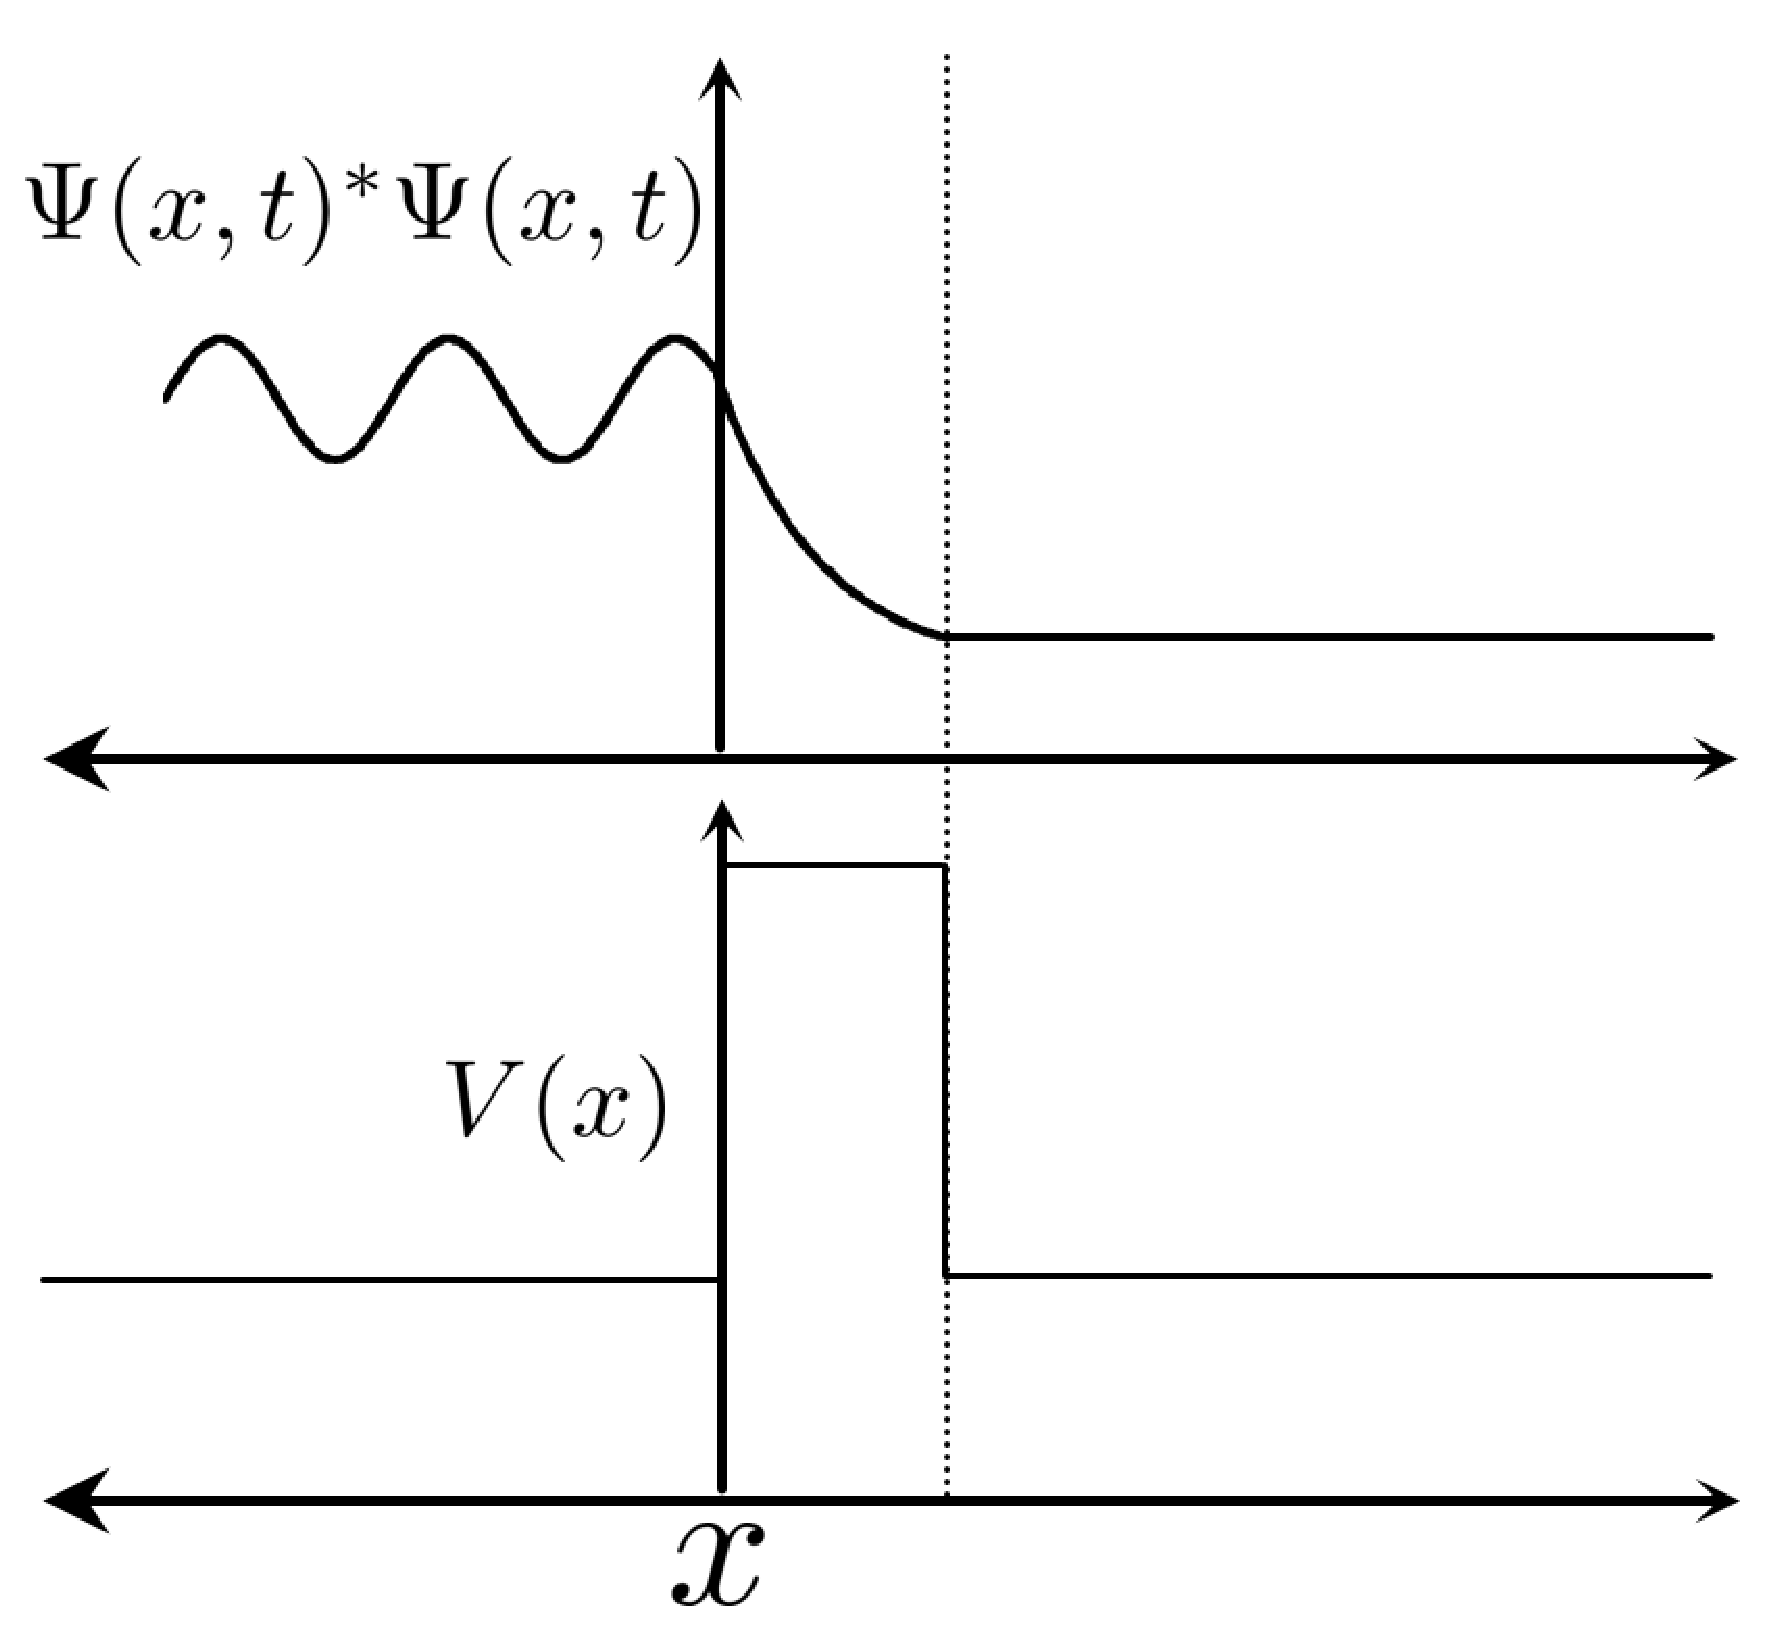
\includegraphics[width = 3.2in]{figures/tunneling_ex.eps}
		\end{center}
		\caption{(Bottom) A simple step potential in one dimension. (Top) The probability density function of a generic quantum system in the presence of a potential energy step barrier. There is an exponential decrease in probability through the barrier, and a uniform probability beyond the barrier.}
		
		\label{fig:quantum_tunneling}
	\end{figure}
	
	\subsection{Quantum Annealing}
	
	Quantum annealing is the use of quantum, rather than thermal fluctuations to traverse the free energy landscape of a system. This is accomplished by introducing an additional Hamiltonian term that does not commute with the classical Hamiltonian. The term is introduced to account for the presence of a tunneling field which controls the frequency with which quantum fluctuations occur in the system. In effect, this term controls the relative importance of quantum effects on the behavior of the modeled system. This term, much like thermal energy in simulated annealing, is gradually reduced over the course of the simulation \cite{das2005qakcs}. The time dependent Schrödinger equation \footnote{Note that the presence of the Schrödinger equation in section does not imply that quantum annealing requires the annealed system must be an approximation to a wavefunction. It merely serves as an exposition of the properties of physical system which is modeled.} for such a system has the form \cite{mukherjee2015multivariatesearchqa}: \begin{equation}
	[\lambda(t)H' + H_0]\psi = i\hbar \frac{\partial \psi}{\partial t}
	\end{equation} where \begin{math} \lambda(t) \end{math} is the time-variance function of the tunneling field, \begin{math} H' \end{math} is the Hamiltonian term describing the tunneling field, and \begin{math} H_0 \end{math} is the classical Hamiltonian. 
	
	The fluctuations induced by the tunneling field are tunneling events, which transition the system from one configuration to a different, lower-energy configuration directly, without assuming any of the higher energy configurations between the two. Said differently, the quantum tunneling field enables the penetration of energy barriers. The addition of these quantum fluctuations also ensures that each possible state of the system can be reached \cite{das2005qakcs}. 
	
	% Strictly speaking, this document does not claim to describe a quantum annealing process as it is presented in the referenced literature. 
	
	% There is a great deal of academic writing describing QA in the language of physics, but very little writing describing the concept from an algorithmic perspective. For this reason, and because there are significant differences between the artificial simulation of quantum-inspired annealing and the physical phenomenon which is being approximated, a new terminology is proposed. In this document, a new more specific term is introduced in order to disambiguate.
	
	% Simulated quantum annealing (SQA) is the quantum mechanical counterpart of simulated thermal annealing. Like simulated thermal annealing, simulated quantum annealing is a global search algorithm which seeks the global minimum of a cost function in a configuration space. 
	
	% In continuously oscliating annealing schedules, consistently good states will tend to attract the search. Bad states will be randomly visited. Partition the space of states into for each synapse into discrete bins. Track the number of times a bin is hit by the search for each synapse. Given enough time and suffiently small bins, the modes of each histogram will come to represent the global minima.
	
	
	\section{Notation and Terminology Conventions}
	
	There is a great deal of academic writing describing quantum annealing in the language of physics, but very little writing describing the concept from an algorithmic perspective. For this reason a new, more specific term is introduced in this document. Simulated quantum annealing (SQA) is the quantum mechanical counterpart of simulated thermal annealing. 
	
	% [Physics to Algorithmic translation table]
	% Free Energy Surface - Error Manifold - Cost Function
	% System Configuration -  
	
	The term neuron will be used in this document to describe the information processing elements of a neural network. This convention is selected both for conciseness and for the useful adjectival form, neural, which will be of great explanatory utility in the coming chapters.
	
	
	%Read (Haykin pg 561) Table 11.1
	
	
	\chapter{Methodology}
	
	\section{Simulated Annealing}
	
	\section{Neighborhood Functions: Traversing the Cost Surface}
	
	The SA algorithm requires that a neighborhood function, \begin{math} \mathcal{N} \end{math}, be specified to produce new solutions from a given solution. The neighborhood function performs the search of the solution space, as it specifies new solutions which can be either accepted or rejected according to the acceptance criteria. Thus, \begin{math} \mathcal{N} \end{math} determines how the algorithm traverses the cost surface of the problem. A traversal action, or move, on a surface, may be decomposed into two components: the distance moved and the direction of the move. These components may be specified independently of one another. The distance of the move on the cost surface has been examined in previous work \cite{szu1987fastsimulatedannealing,tsallis1996generalizedsimulatedannealing}, and is often specified using a \textit{visiting distribution}, which is defined as a probability distribution over the move distance parameter. The visiting distribution specifies the magnitude of the move, but does not specify anything about the direction of the move. 
	
	The direction of a cost surface traversal is the allocation of the total move distance to each of the possible traversal dimensions. A traversal dimension, or degree of freedom, is a solution parameter which can be modified by the SA algorithm. In previous work [need several citations here]\cite{}, the move distance has been applied isotropically in all possible dimensions of travel. In physical science, isotropicity is phenomenological property of being uniformly applicable in all dimensions. In the context of neighborhood functions this means that the total distance moved in each of the possible travel dimensions is equal in magnitude, and random in sign. In the following sections a novel method is developed for applying the cost surface traversal distance anisotropically. 
	
	For the following sections, an arbitrary, simple problem will be used to demonstrate these concepts.
	
	In the following sections several realizations of a neighborhood function are presented. 
	
	\subsection{Visiting Distributions}
	
	[graphics stub: all of the visiting distributions considered in this paper.]
	
	To understand the origin of this advantage, it is instructive to contrast equations \ref{eq:thermal_traversal_prob} and \ref{eq:quantum_tunneling_prob}. Both describe the same value, but the importance of the width and height of the traversed barrier in the two equations is considerably different. For systems in which quantum tunneling is possible, the probability of penetrating a barrier of height \begin{math} \Delta V \end{math} is increased by a factor of approximately \begin{math} e^{\Delta V} \end{math}, for large values of \begin{math} \Delta V \end{math}. This relationship is depicted graphically in Fig.~\ref{fig:quantum_advantage} which shows the probability of barrier traversal for a system which allows quantum fluctuations, divided by the same probability for a system which only considers thermal fluctuations. Therefore, physical models which considers quantum effects are much more likely to predict penetration of tall, thin energy barriers than those which only include classical thermal effects.
	
	\begin{figure}[ht!]
		
		\begin{minipage}[b]{0.48\linewidth}
			\centering
			\centerline{\epsfig{figure=figures/quantum_advantage_a.eps,width=7cm}}
			%  \vspace{2.0cm}
			\centerline{(a)}\medskip
		\end{minipage}
		\hfill
		\begin{minipage}[b]{0.48\linewidth}
			\centering
			\centerline{\epsfig{figure=figures/quantum_advantage_b.eps,width=7cm}}
			%  \vspace{2.0cm}
			\centerline{(b)}\medskip
		\end{minipage}
		%\vspace{-0.5cm}
		\caption{
			(a) A potential energy barrier on a one-dimensional potential energy surface.
			(b) The tunneling probability relative to the probability of traversal due to thermal fluctuation for a step barrier plotted as a function of the height and width of the barrier.}
		\label{fig:quantum_advantage}
		%
	\end{figure}
	
	
	\subsubsection{Gaussian}
	
	
	
	An SA algorithm using a Gaussian visiting distribution is often called classical simulated annealing (CSA).
	
	
	\subsubsection{Exponential}
	
	\subsubsection{Cauchy}
	
	\subsubsection{Uniform}
	
	\subsection{Anisotropicity}
	
	
	
	\subsubsection{Isotropic Anisotropicity}
	\subsubsection{Uniform Anisotropicity}
	\subsubsection{Variable Anisotropicity}
	
	
	
	\section{Feed-Forward Neural Network Representation}
	
	With the feed-forward neural network problem representation described in sections \ref{eq:boltzmannDist}-\ref{eq:boltzmannDist}, and the description of SA 
	
	% http://math.stackexchange.com/questions/484395/how-to-generate-a-cauchy-random-variable
	% https://en.wikipedia.org/wiki/Inverse_transform_sampling
	
%	It is shown in Proof [n] that this algorithm is certain to eventually find the minimum possible
	
	%formal proof of the eventual optimality of the simulated quantum annealing algorithm

	
	
	
	%[After discussing the way in which the algorithm is implemented] ...The net effect of this design is to allow the algorithm to move from a local minima configuration, to a different, lower-error configuration, without requiring the evaluation of intervening, higher-error configurations. This means that the probability of "tunneling" to a state
	
	
	
	
	\chapter{Results}
	
%	Is my algorithm computationally efficient as in Haykin, pg 229?
	\chapter{Conclusion}
	
	
	\appendix		% Appendix begins here
	
	\chapter{First appendix title}
	
	\section{In an appendix} 
	
	This is appendix section A.1.
	
	Note: I highly recommend you create each chapter in a separate file
	including the \verb|\chapter| command and \verb|\include| the file.
	Then you can use \verb|\includeonly| to process selected chapters and
	you avoid having to latex/preview/print your entire document every
	time.
	
	%\begin{Bibliography}	     % CAUTION: the first B is capital B.
	%\bibitem[key] A listing ... % You can also use the `thebibliography'
	%\bibitem[key2] A another    % environment described in LaTeX manual.
	%\bibitem[key3]...	     % The usages of \bibitem and \cite{..} are
	%\end{Bibliography}          % explained in Section 4.3 of the LaTeX manual.
	
	% you can also use BibTeX instead of the above as I have done below. 
	% see the LaTeX manual and the
	% documentation available from /usr/TeX/doc.  There is an AFIT 
	% bibliography style called thesnumb.  It has some special types 
	% and fields.  See some sample entries and info in thesnumb.doc.  
	% Note: thisthesis bibliography style only works with bibtex 
	% version .99a or higher.
	
	\bibliographystyle{thesnumb}
	\bibliography{synapticAnnealingBib}
	
	\begin{vita}
		Insert your brief biographical sketch here. Your permanent
		address is generated automatically.
	\end{vita}
	
	%\begin{vita} %uncomment for twoauthor option
	%	The second vita.
	%	Insert the second authors brief biographical sketch here. 
	%\end{vita}
	
\end{document}

% Please mail your suggestions and complaints to jdyoung@afit.af.mil.
